\section{1174008 - Arjun Yuda Firwanda}
\subsection{Soal Teori}
\begin{enumerate}

	\item Jelaskan apa itu random forest, sertakan gambar ilustrasi buatan sendiri.
	\hfill\break
	Random Forest merupakan suatu metode penyelesaian permasalahan. Metode Random Forest sebagai sebutan metode Decision Tree atau metode yang menyerupai pohon pengambilan keputusan sebuah diagram air yang memiliki sebuah root node yang digunakan untuk mengumpulkan suatu data.

	\begin{figure}[H]
	\centering
		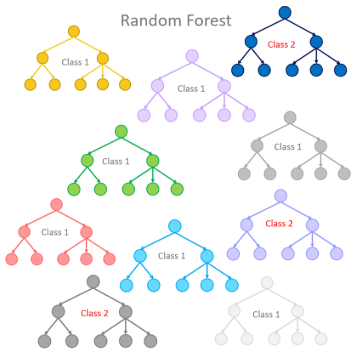
\includegraphics[width=4cm]{figures/1174008/3/teori/RandomForest.PNG}
		\caption{Random Forest.}
	\end{figure}

	\item Jelaskan cara membaca dataset kasus dan artikan makna setiap file dan isi field masing-masing file.
	\hfill\break

	\begin{itemize}
		\item Pertama download dataset terlebih dahulu lalu buka dengan menggunakan software spyder guna melihat isi dari dataset tersebut.

		\item Data tersebut memiliki extensi file bernama .txt dan didalamnya terdapat class dari field.

		\item Misalnya saja pada data jenis burung memiliki file index dan angka, dimana index berisi angka yang memiliki makna berupa jenis burung.

		\item bahkan nama burung sedangkan field memiliki isi nilai berupa 0 dan 1 yang dimana sifatnya boolean atau Ya dan Tidak.

		\item Hal ini dikarenakan komputer hanya dapat membaca bilangan biner maka dari itu field yang di isikan berupa angka.

		\item Artinya angka 0 berarti tidak dan angka 1 berarti Ya.
	\end{itemize}
	
	\item Jelaskan apa itu cross validation.
	\hfill\break
	Cross Validation suatu metode yang menerapkan statistik yang biasanya  dapat digunakan untuk menilai kinerja model serta algoritma, Pada data tersebut dapat dipisahkan menjadi dua bagian subset, seperti data proses pembelajaran dan data validasi atau evaluasi. Selain itu juga Cross Validation ini dapat digunakan dikarenakan mampu mengurangi waktu komputasi dengan tetap serta dapat menjaga keakuratan estimasi.
	\begin{figure}[H]
	\centering
		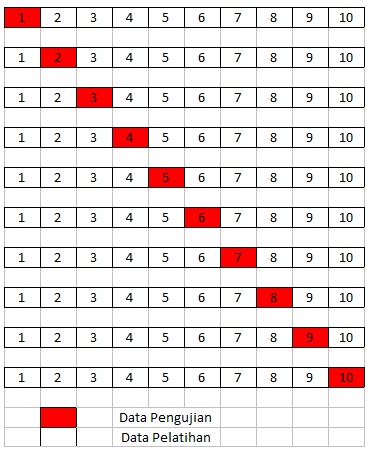
\includegraphics[width=4cm]{figures/1174008/3/teori/CrossValidation.PNG}
		\caption{Random Forest.}
	\end{figure}

	\item Jelaskan apa arti score 44 \% pada random forest, 27\% pada decission tree dan 29 \% dari SVM.
	\hfill\break
	Dimana Score 44 \% diperoleh dari hasil pengelohan dataset jenis burung. Dimana akan dilakukan proses pembagian data testing dan data training lalu diproses dan menghasilkan score sebanyak 44 \% dimana menjelaskan bahwa score tersebut digunakan sebagai pembanding dalam tingkat keakuratannya. Pada dicision tree akan memperoleh data lebih kecil yaitu sebanyak 27 \% hal ini dikarenakan data yang diolah menggunakan dicision tree dibagi menjadi beberapa tree dan lalu disimpulkan untuk mendapatkan data yang akurat. Pada SVM akan memperoleh score sebanyak 29 \% hal ini dikarenakan data yang dimiliki masih bernilai netral sehingga tingkat keakuratannya masih belum jelas.

	\item Jelaskan bagaimana cara membaca confusion matriks dan contohnya memakai gambar atau ilustrasi sendiri.
	\hfill\break
	Confusion Matrix atau error matrix yang dapat memberikan informasi perbandingan hasil klasifikasi sebenarnya. Confusion Matrix berbentuk tabel matriks yang menggambarkan kinerja model klasifikasi pada serangkaian data uji yang nilai sebenarnya telah diketahui.

	\begin{figure}[H]
	\centering
		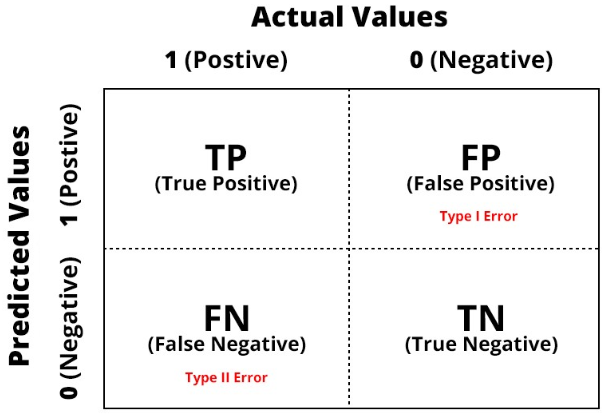
\includegraphics[width=4cm]{figures/1174008/3/teori/ConfusionMatrix.PNG}
		\caption{Random Forest.}
	\end{figure}

	\item Jelaskan apa itu voting pada random forest disertai dengan ilustrasi gambar sendiri
	\hfill\break
	Voting pada random forest ialah sebuah proses pemilihan dari tree yang dimana akan dimunculkan hasilnya dan disimpulkan menjadi informasi yang pasti. Penentuan klasifikasi menguunakan metode random forest diambil berdasarkan hasil voting dari decision tree yang terbentuk. Setelah decision tree atau pohon terbentuk, maka akan dilakukan voting pada setiap kelas dari data sampel. Kemudian, selanjutnya mengkombinasikan vote dari setiap kelas kemudian diambil vote yang paling banyak. Dengan menggunakan metode penyelesaian random forest pada klasifikasi data maka, akan menghasilkan vote yang paling baik.

	\begin{figure}[H]
	\centering
		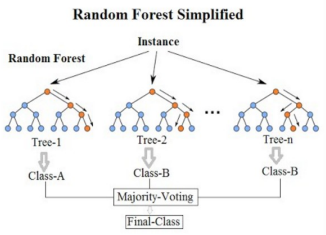
\includegraphics[width=4cm]{figures/1174008/3/teori/VotingRandomForest.PNG}
		\caption{Random Forest.}
	\end{figure}
\end{enumerate}


\subsection{Praktek Program}
\begin{enumerate}
	\item Buat aplikasi sederhana menggunakan pandas dan jelaskan arti setiap baris kode yang dibuat(harus beda dengan teman sekelas).
	\hfill\break
	\lstinputlisting[firstline=1, lastline=5]{src/1174008/3/123.py}
	Kode di atas digunakan untuk mengimpor atau mengirim library pandas sebagai Arjun, Hasilnya adalah sebagai berikut :
	\begin{figure}[H]
	\centering
		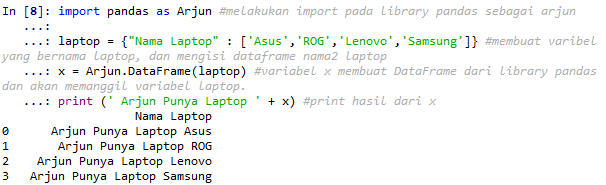
\includegraphics[width=4cm]{figures/1174008/3/teori/hasilsoal1.PNG}
		\caption{Hasil Soal 1.}
	\end{figure}

	\item buat aplikasi sederhana menggunakan numpy dan jelaskan arti dari setiap baris kode yang dibuat(harus beda dengan teman sekelas)
	\hfill\break
	\lstinputlisting[firstline=11, lastline=16]{src/1174008/3/123.py}
	Fungsi eye disini berguna untuk memanggil matrix identitas dengan jumlah colom dan baris sesuai yang ditentukan. Disini saya telah menentukan 10 colom dan baris maka dari itu hasilnya akan memunculkan matrix identitas 10x10, Hasilnya adalah sebagai berikut :
	\begin{figure}[H]
	\centering
	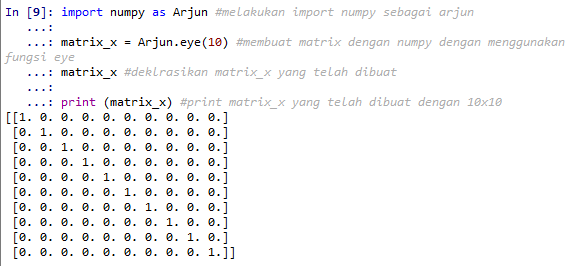
\includegraphics[width=4cm]{figures/1174008/3/teori/hasilsoal2.PNG}
		\caption{Hasil Soal 2.}
	\end{figure}
	
	\item buat aplikasi sederhana menggunakan matplotlib dan jelaskan arti dari setiap baris kode(harus beda dengan teman sekelas)
	\hfill\break
	\lstinputlisting[firstline=21, lastline=26]{src/1174008/3/123.py}
	Jalankan source code diatas dengan spyder atau anaconda sehingga hasilnya akan seperti berikut : 

	\begin{figure}[H]
	\centering
		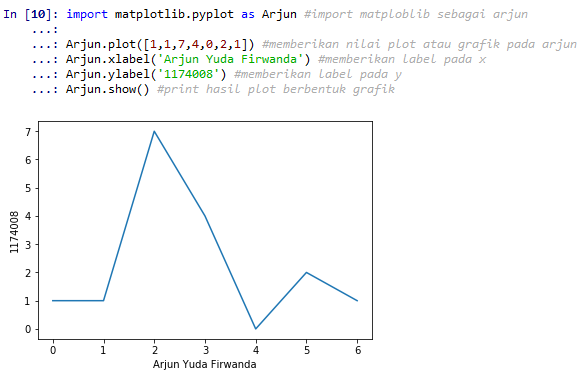
\includegraphics[width=4cm]{figures/1174008/3/teori/hasilsoal3.PNG}
		\caption{Hasil Soal 3.}
	\end{figure}

%mulai nomor 4

	\item jalankan program klasifikasi Random Forest pada bagian teori bab ini. Tunjukkan keluarannya dari komputer sendiri dan artikan maksud setiap luaran yang didapatkan.
	\hfill\break
\begin{itemize}
	\item Source Code pertama pada random forest berfungsi untuk membaca dataset yang memiliki format text file dengan mendefinisikan variabel yang bernama imgatt. Variabel tersebut berisi value untuk membaca data. 
	\lstinputlisting[firstline=2, lastline=9]{src/1174008/3/tugas3.py}
	Hasilnya adalah seperti ini :

	\begin{figure}[H]
	\centering
		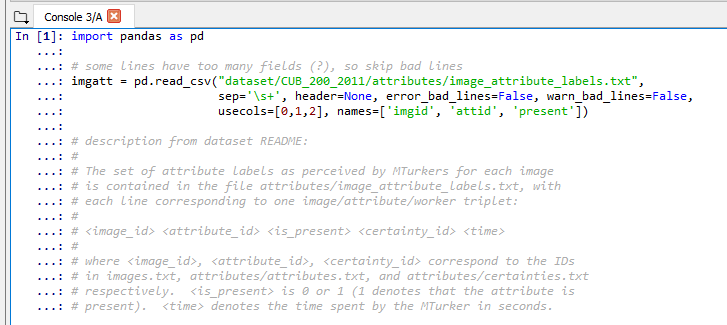
\includegraphics[width=4cm]{figures/1174008/3/praktek/soal41.PNG}
		\caption{Hasil Soal 4 - 1}
	\end{figure}

	\item Pada source code berikutnya akan mengembalikan baris teratas dari DataFrame variabel imgatt.
	\lstinputlisting[firstline=11, lastline=13]{src/1174008/3/tugas3.py}
	Hasilnya adalah seperti ini :

	\begin{figure}[H]
	\centering
		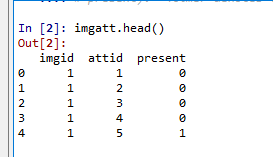
\includegraphics[width=4cm]{figures/1174008/3/praktek/soal42.PNG}
		\caption{Hasil Soal 4 - 2}
	\end{figure}

	\item Pada output berikutnya akan menampilkan jumlah kolom dan baris dari DataFrame imgatt. 
	\lstinputlisting[firstline=16, lastline=18]{src/1174008/3/tugas3.py}
	Hasilnya adalah seperti ini :

	\begin{figure}[H]
	\centering
		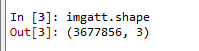
\includegraphics[width=4cm]{figures/1174008/3/praktek/soal43.PNG}
		\caption{Hasil Soal 4 - 3}
	\end{figure}

	\item Variabel imgatt2 telah menggunakan function yang bernama pivot guna mengubah kolom jadi baris dan sebaliknya dari DataFrame sebelumnya.
	\lstinputlisting[firstline=21, lastline=23]{src/1174008/3/tugas3.py}
	Hasilnya adalah seperti ini :

	\begin{figure}[H]
	\centering
		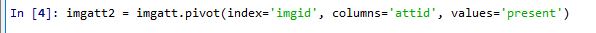
\includegraphics[width=4cm]{figures/1174008/3/praktek/soal44.PNG}
		\caption{Hasil Soal 4 - 4}
	\end{figure}

	\item Variabel imgatt2 head berfungsi untuk mengembalikan value teratas pada DataFrame imgatt2.
	\lstinputlisting[firstline=26, lastline=28]{src/1174008/3/tugas3.py}
	Hasilnya adalah seperti ini :

	\begin{figure}[H]
	\centering
		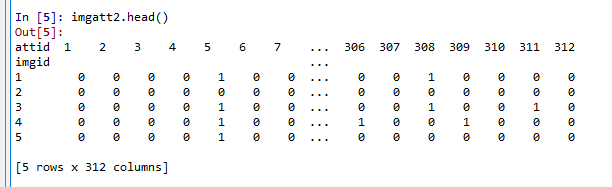
\includegraphics[width=4cm]{figures/1174008/3/praktek/soal45.PNG}
		\caption{Hasil Soal 4 - 5}
	\end{figure}

	\item Menghasilkan jumlah kolom dan baris pada DataFrame imgatt2.
	\lstinputlisting[firstline=31, lastline=33]{src/1174008/3/tugas3.py}
	Hasilnya adalah seperti ini :

	\begin{figure}[H]
	\centering
		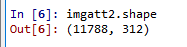
\includegraphics[width=4cm]{figures/1174008/3/praktek/soal46.PNG}
		\caption{Hasil Soal 4 - 6}
	\end{figure}

	\item Menunjukkan dalam melakukan pivot yang mana imgid menjadi sebuah index yang unik.
	\lstinputlisting[firstline=36, lastline=41]{src/1174008/3/tugas3.py}
	Hasilnya adalah seperti ini :

	\begin{figure}[H]
	\centering
		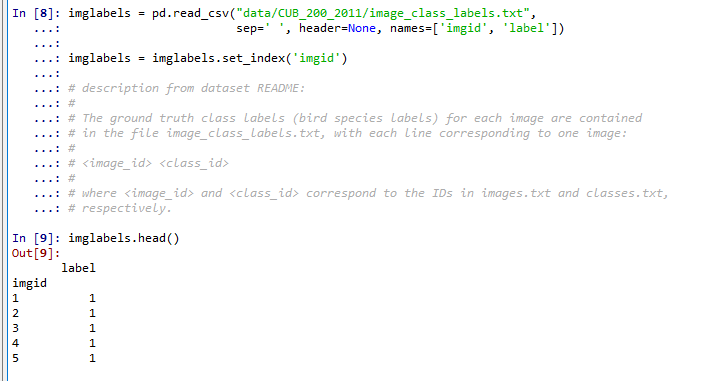
\includegraphics[width=4cm]{figures/1174008/3/praktek/soal47.PNG}
		\caption{Hasil Soal 4 - 7}
	\end{figure}

	\item Akan melakukan load jawabannya yang berisi apakah burung tersebut termasuk spesies yang mana. Kolom tersebut yaitu imgid dan label.
	\lstinputlisting[firstline=44, lastline=46]{src/1174008/3/tugas3.py}
	Hasilnya adalah seperti ini :

	\begin{figure}[H]
	\centering
		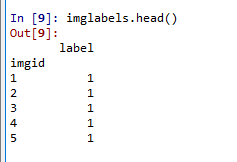
\includegraphics[width=4cm]{figures/1174008/3/praktek/soal48.PNG}
		\caption{Hasil Soal 4 - 8}
	\end{figure}

	\item Menunjukkan bahwa jumlah baris sebanyak 11788 dan kolom 1 yang dimana kolom tersebut adalah jenis spesies pada burung.
	\lstinputlisting[firstline=49, lastline=51]{src/1174008/3/tugas3.py}
	Hasilnya adalah seperti ini :

	\begin{figure}[H]
	\centering
		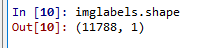
\includegraphics[width=4cm]{figures/1174008/3/praktek/soal49.PNG}
		\caption{Hasil Soal 4 - 9}
	\end{figure}

	\item Melakukan join antara imgatt2 dengan imglabels dikarenakan memiliki isi yang sama sehingga akan mendapatkan sebuah data ciri-ciri dan data jawaban sehingga bisa dikategorikan sebagai supervised learning.
	\lstinputlisting[firstline=54, lastline=57]{src/1174008/3/tugas3.py}
	Hasilnya adalah seperti ini :

	\begin{figure}[H]
	\centering
		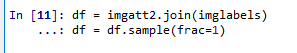
\includegraphics[width=4cm]{figures/1174008/3/praktek/soal410.PNG}
		\caption{Hasil Soal 4 - 10}
	\end{figure}

	\item Melakukan drop pada label yang ada didepan dan akan menggunakan label yang baru di joinkan.
	\lstinputlisting[firstline=60, lastline=63]{src/1174008/3/tugas3.py}
	Hasilnya adalah seperti ini :

	\begin{figure}[H]
	\centering
		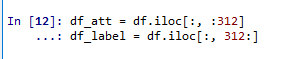
\includegraphics[width=4cm]{figures/1174008/3/praktek/soal411.PNG}
		\caption{Hasil Soal 4 - 11}
	\end{figure}

	\item Mengecek isi 5 data teratas pada df att.
	\lstinputlisting[firstline=66, lastline=68]{src/1174008/3/tugas3.py}
	Hasilnya adalah seperti ini :

	\begin{figure}[H]
	\centering
		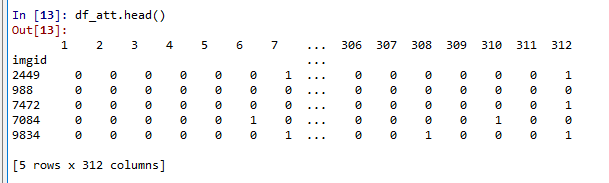
\includegraphics[width=4cm]{figures/1174008/3/praktek/soal412.PNG}
		\caption{Hasil Soal 4 - 12}
	\end{figure}

	\item Mengecek isi data teratas dari df label.
	\lstinputlisting[firstline=71, lastline=73]{src/1174008/3/tugas3.py}
	Hasilnya adalah seperti ini :

	\begin{figure}[H]
	\centering
		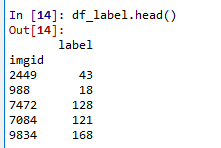
\includegraphics[width=4cm]{figures/1174008/3/praktek/soal413.PNG}
		\caption{Hasil Soal 4 - 13}
	\end{figure}

	\item Membagi 8000 row pertama menjadi data training dan sisanya adalah data testing.
	\lstinputlisting[firstline=76, lastline=84]{src/1174008/3/tugas3.py}
	Hasilnya adalah seperti ini :

	\begin{figure}[H]
	\centering
		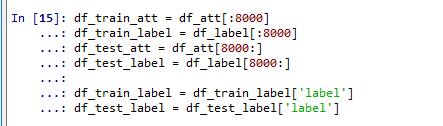
\includegraphics[width=4cm]{figures/1174008/3/praktek/soal414.PNG}
		\caption{Hasil Soal 4 - 14}
	\end{figure}

	\item Pemanggilan class RandomForestClassifier. Dimana artinya menunjukkan banyak kolom pada setiap tree adalah 50.
	\lstinputlisting[firstline=87, lastline=90]{src/1174008/3/tugas3.py}
	Hasilnya adalah seperti ini :

	\begin{figure}[H]
	\centering
		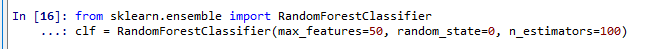
\includegraphics[width=4cm]{figures/1174008/3/praktek/soal415.PNG}
		\caption{Hasil Soal 4 - 15}
	\end{figure}

	\item Menunjukkan hasil prediksi dari Random Forest.
	\lstinputlisting[firstline=93, lastline=95]{src/1174008/3/tugas3.py}
	Hasilnya adalah seperti ini :

	\begin{figure}[H]
	\centering
		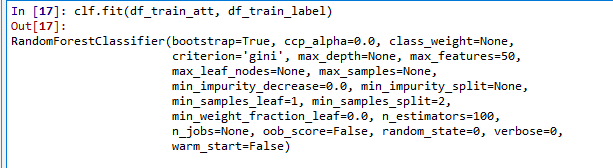
\includegraphics[width=4cm]{figures/1174008/3/praktek/soal416.PNG}
		\caption{Hasil Soal 4 - 16}
	\end{figure}

	\item Menampilkan besaran akurasi dari prediksi pada Random Forest yang merupakan score perolehan klarifikasi.
	\lstinputlisting[firstline=98, lastline=100]{src/1174008/3/tugas3.py}
	Hasilnya adalah seperti ini :

	\begin{figure}[H]
	\centering
		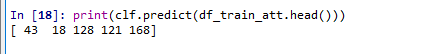
\includegraphics[width=4cm]{figures/1174008/3/praktek/soal417.PNG}
		\caption{Hasil Soal 4 - 17}
	\end{figure}

	\item Menampilkan besaran akurasi dari prediksi pada Random Forest yang merupakan score perolehan klarifikasi.
	\lstinputlisting[firstline=103, lastline=105]{src/1174008/3/tugas3.py}
	Hasilnya adalah seperti ini :

	\begin{figure}[H]
	\centering
		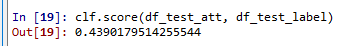
\includegraphics[width=4cm]{figures/1174008/3/praktek/soal418.PNG}
		\caption{Hasil Soal 4 - 18}
	\end{figure}
\end{itemize}

%Mulai nomor 5

\item Jalankan program confusion matrix pada bagian teori bab ini. Tunjukkan keluarannya dari komputer sendiri dan artikan maksud setiap luaran yang didapatkan.
\hfill\break

\begin{itemize}
	\item Melakukan import confusion matrix pada library sklearn matriks.
	\lstinputlisting[firstline=108, lastline=112]{src/1174008/3/tugas3.py}
	Hasilnya adalah seperti ini :

	\begin{figure}[H]
	\centering
		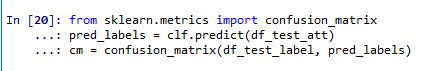
\includegraphics[width=4cm]{figures/1174008/3/praktek/soal51.PNG}
		\caption{Hasil Soal 5 - 1}
	\end{figure}

	\item Menampilkan isi cm dalam bentuk matrix yang berupa array.
	\lstinputlisting[firstline=115, lastline=117]{src/1174008/3/tugas3.py}
	Hasilnya adalah seperti ini :

	\begin{figure}[H]
	\centering
		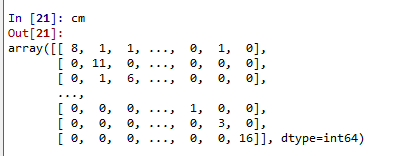
\includegraphics[width=4cm]{figures/1174008/3/praktek/soal52.PNG}
		\caption{Hasil Soal 5 - 2}
	\end{figure}

	\item Membuat dan menampilkan hasil plot.
	\lstinputlisting[firstline=120, lastline=166]{src/1174008/3/tugas3.py}
	Hasilnya adalah seperti dibawah ini :

	\begin{figure}[H]
	\centering
		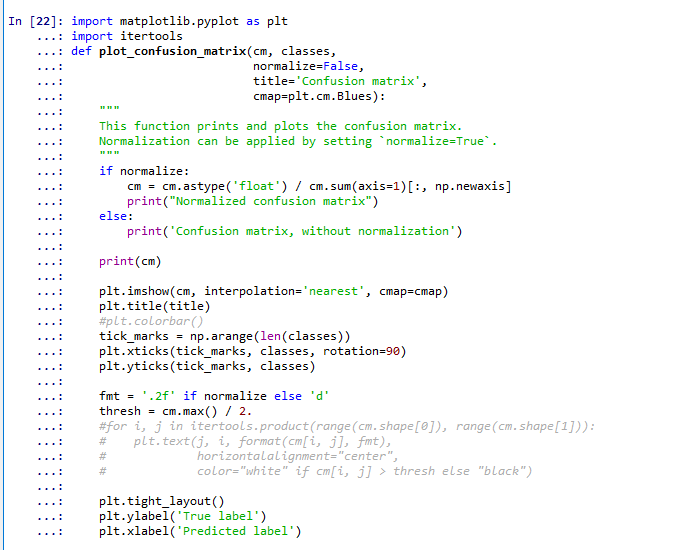
\includegraphics[width=4cm]{figures/1174008/3/praktek/soal5_3.PNG}
		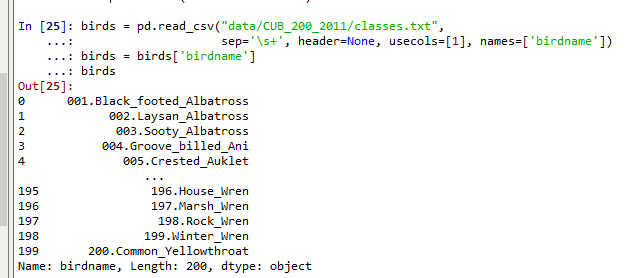
\includegraphics[width=4cm]{figures/1174008/3/praktek/soal56.PNG}
		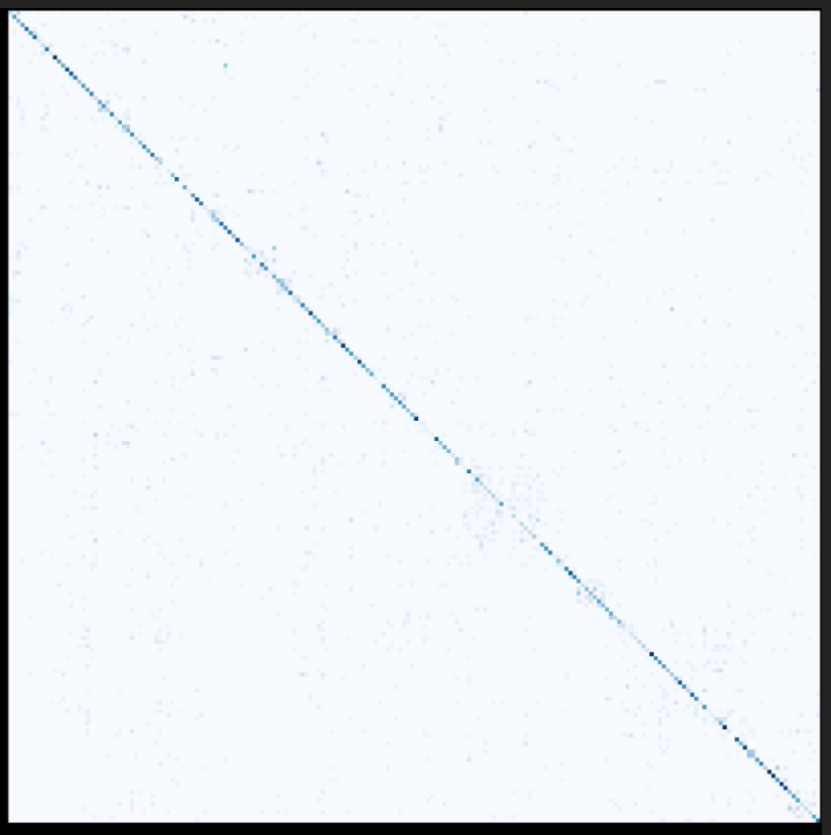
\includegraphics[width=4cm]{figures/1174008/3/praktek/2.PNG}
		\caption{Menampilkan hasil plot}
	\end{figure}

\end{itemize}

%mulai soal nomor 6

\item Jalankan program klasifikasi SVM dan Decission Tree pada bagian teori bab ini. Tunjukkan keluarannya dari komputer sendiri dan artikan maksud setiap luaran yang didapatkan.
	\hfill\break
\begin{itemize}
	\item Menunjukkan klarifikasi dengan decission tree menggunakan dataset yang sama dan akan memunculkan akurasi prediksi.
	\lstinputlisting[firstline=169, lastline=174]{src/1174008/3/tugas3.py}
	Hasilnya adalah seperti ini :

	\begin{figure}[H]
	\centering
		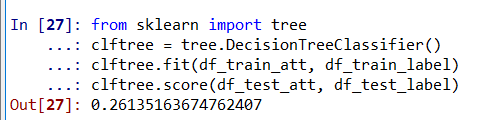
\includegraphics[width=4cm]{figures/1174008/3/praktek/soal61.PNG}
		\caption{Hasil Soal 6 - 1}
	\end{figure}

	\item Menunjukkan klarifikasi dengan SVM menggunakan dataset yang sama dan akan memunculkan akurasi prediksi.
	\lstinputlisting[firstline=177, lastline=182]{src/1174008/3/tugas3.py}
	Hasilnya adalah seperti ini :

	\begin{figure}[H]
	\centering
		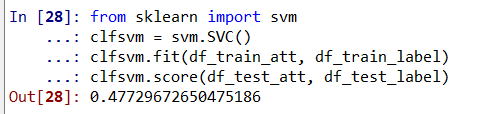
\includegraphics[width=4cm]{figures/1174008/3/praktek/soal62.PNG}
		\caption{Hasil Soal 6 - 2}
	\end{figure}
\end{itemize}

%mulai soal nomor 7

\item Jalankan program cross validaiton pada bagian teori bab ini. Tunjukkan keluarannya dari komputer sendiri dan artikan maksud setiap luaran yang didapatkan.
	\hfill\break
\begin{itemize}
	\item Menunjukkan hasil cross validation pada Random Forest.
	\lstinputlisting[firstline=185, lastline=189]{src/1174008/3/tugas3.py}
	Hasilnya adalah seperti ini :

	\begin{figure}[H]
	\centering
		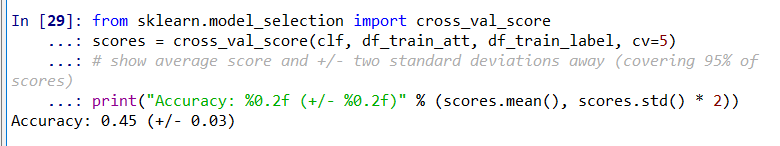
\includegraphics[width=4cm]{figures/1174008/3/praktek/soal71.PNG}
		\caption{Hasil Soal 7 - 1}
	\end{figure}

	\item Menunjukkan hasil cross validation pada Desiccion Tree.
	\lstinputlisting[firstline=192, lastline=195]{src/1174008/3/tugas3.py}
	Hasilnya adalah seperti ini :

	\begin{figure}[H]
	\centering
		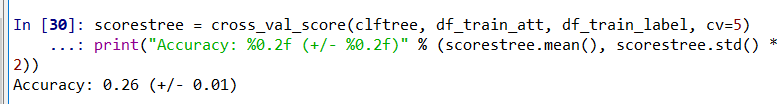
\includegraphics[width=4cm]{figures/1174008/3/praktek/soal72.PNG}
		\caption{Hasil Soal 7 - 2}
	\end{figure}

	\item Menunjukkan hasil cross validation pada SVM.
	\lstinputlisting[firstline=198, lastline=201]{src/1174008/3/tugas3.py}
	Hasilnya adalah seperti ini :

	\begin{figure}[H]
	\centering
		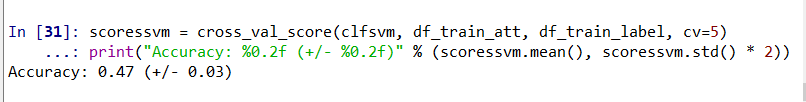
\includegraphics[width=4cm]{figures/1174008/3/praktek/soal73.PNG}
		\caption{Hasil Soal 7 - 3}
	\end{figure}
\end{itemize}

%mulai soal nomor 8

\item Jalankan program pengamatan komponen informasi pada bagian teori bab ini. Tunjukkan keluarannya dari komputer sendiri dan artikan maksud setiap luaran yang didapatkan.
	\hfill\break
\begin{itemize}
	\item Menunjukkan informasi-informasi tree yang dibuat.
	\lstinputlisting[firstline=204, lastline=220]{src/1174008/3/tugas3.py}
	Hasilnya adalah seperti ini :

	\begin{figure}[H]
	\centering
		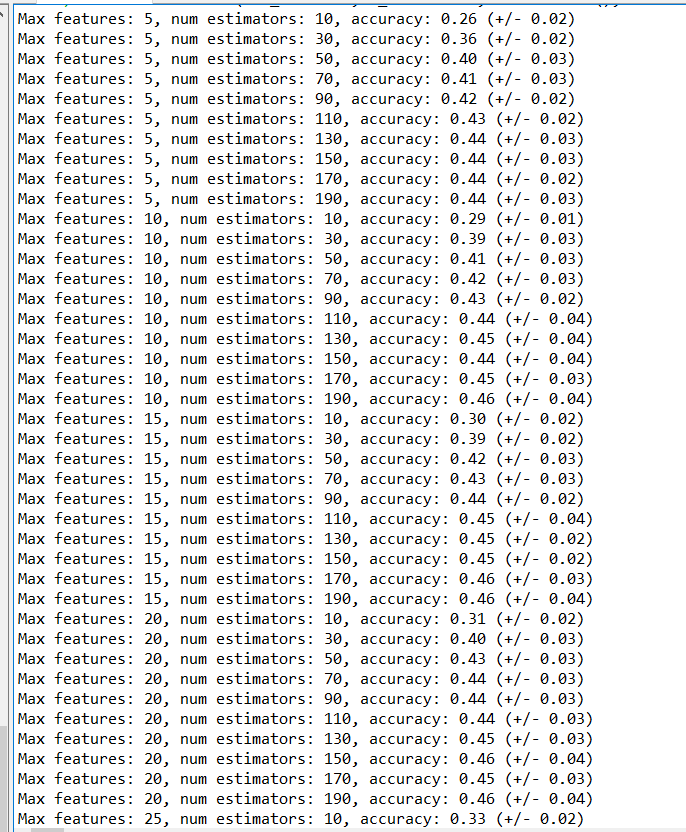
\includegraphics[width=4cm]{figures/1174008/3/praktek/soal81.PNG}
		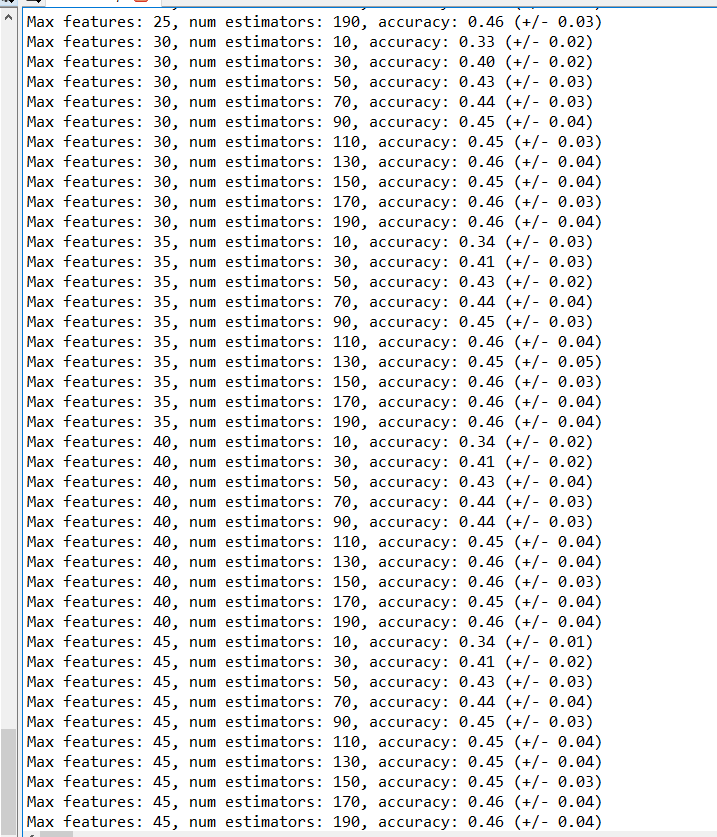
\includegraphics[width=4cm]{figures/1174008/3/praktek/soal82.PNG}
		\caption{Hasil Soal 8 - 1}
	\end{figure}

	\item Menunjukkan hasil dari plotting komponen informasi sehingga dapat kita baca sebagai grafik 3D.
	\lstinputlisting[firstline=222, lastline=238]{src/1174008/3/tugas3.py}
	Hasilnya adalah seperti ini:

	\begin{figure}[H]
	\centering
		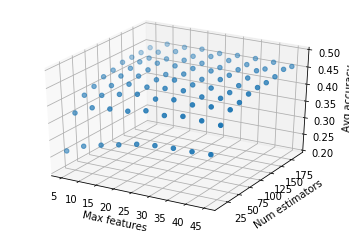
\includegraphics[width=4cm]{figures/1174008/3/praktek/soal83.PNG}
		\caption{Hasil Soal 8 - 2}
	\end{figure}
\end{itemize}
\end{enumerate}


\subsection{Penanganan Error}
\begin{enumerate}
	\item ScreenShoot Error
	\begin{figure}[H]
		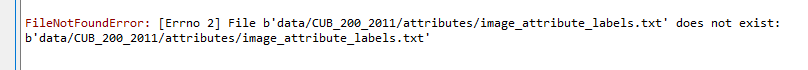
\includegraphics[width=4cm]{figures/1174008/3/error/error.PNG}
		\centering
		\caption{FileNotFoundError}
	\end{figure}
	\item Tuliskan Kode Error dan Jenis Error
	\begin{itemize}
		\item FileNotFoundError
	\end{itemize}
	\item Cara Penangan Error
	\begin{itemize}
		\item FileNotFoundError
		\hfill\break
		Error terdapat pada kesalahan baca file csv, yang tidak terbaca. Dikarenakan letak file yang dibaca tidak para direktori yang sama. Seharusnya letakkan file di direktori yang sama. 
	\end{itemize}
\end{enumerate}

\subsection{Bukti Tidak Plagiat}
\begin{figure}[H]
\centering
	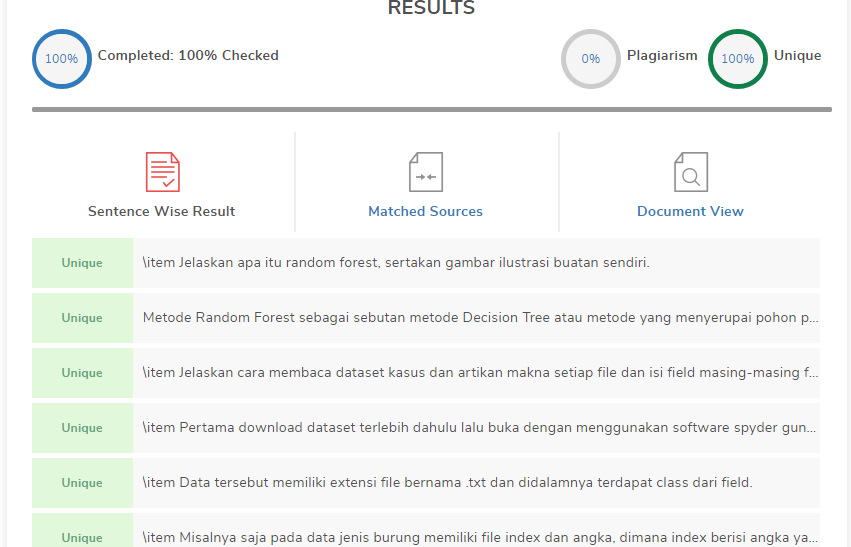
\includegraphics[width=4cm]{figures/1174008/3/buktiplagiat/1.PNG}
	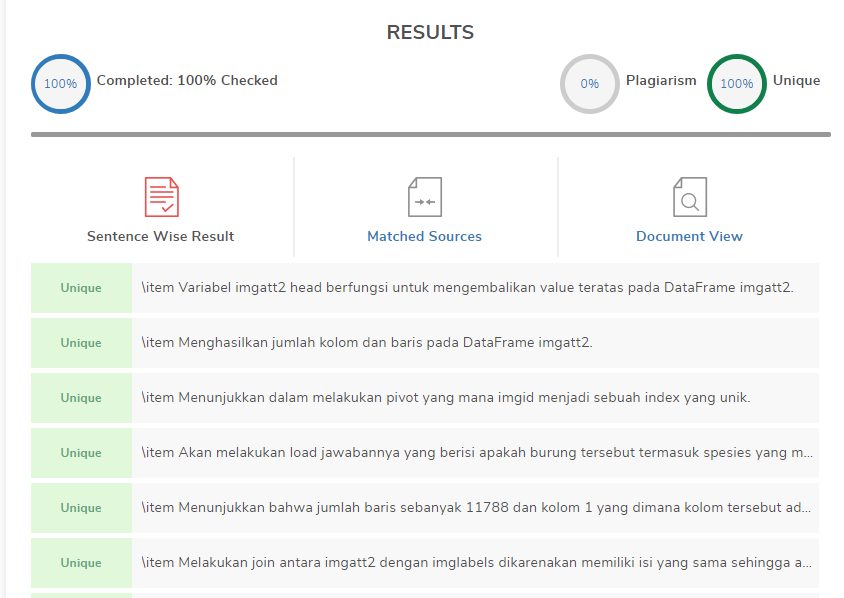
\includegraphics[width=4cm]{figures/1174008/3/buktiplagiat/2.PNG}
	\caption{Bukti Tidak Melakukan Plagiat Chapter 3}
\end{figure}

